% I denne workshop er fokus lidt ændret fra tidligere Workshop. Dette er grundet at tidligere Workshop hovedsageligt havde fokus på projektets login funktionalitet og de dertilhørende usecases. Til denne workshop har gruppen dog vedtaget at det mere oplagt at videre specificere projektets andre dele, her tale om interaktion og implementering.

\section{Indledning}
Fokus er derfor nu på at beskrive hvordan kerne funktionaliteten af en sådan vejrstation kan implementeres, på en hensigtsmæssig måde.\\
Implementationen af vejrstationen skal kunne en række ting. Én af de vigtige ting er, at koden skal kunne acceptere nye sensorer uden store ændringer i koden. Dette kræver en struktur som kan lagre et bredt antal af datatyper. Ydermere skal kommunikationen imellem microcontrolleren og PC-en også kunne operere uafhængigt af hvilken sensor som dataen oprindeligt kommer fra. Denne generalitet i design ligger op til at implementationen burde laves med objekt orienteret programmering. 

\section{Klassediagram}
\begin{figure}[H]
    \centering
    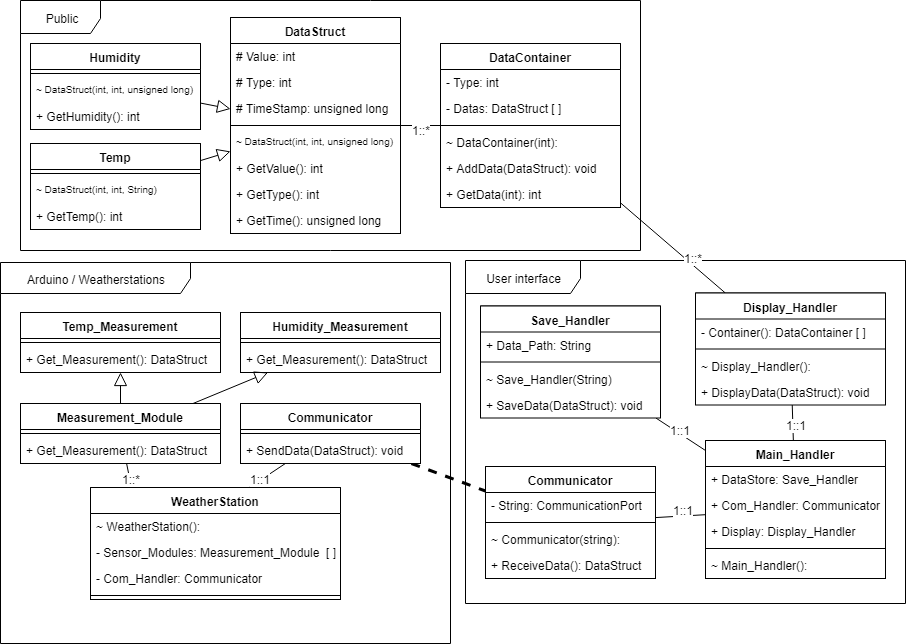
\includegraphics[width=1\textwidth, angle =0]{Struktureret_System_Udvikling/Workshop_2/Assets/Workshop2_ClassDiagram.png}
    \caption{Interaktions klassediagram}
    \label{fig:classdiagram}
\end{figure}

\noindent
Det overstående klassediagram [Figur \ref{fig:classdiagram}] viser implementationen af vejrstationen og dens kommunikation på tværs af klasserne. For overskueligheden skyld er klassediagrammet inddelt i tre generelle kategorier.

\subsection{Public}
\begin{itemize}
    \item[-] \textbf{Humidity og Temp} \hfill \\
    \textit{Humidity} og \textit{Temp} klasserne opbevare forholdsvis et luftfugtighed- og temperaturinput som der hver især bliver sendt videre til klassen \textit{DataStruct}, sammen med et tidspunkt og et type ID. 
    
    \item[-] \textbf{DataStruct} \hfill \\
    \textit{DataStruct} klassen opbevar hver måling fra en given sensor. \textit{DataStruct}'en gemmer værdierne: \textit{Value}, \textit{Type} og \textit{TimeStamp}, alle gemt som \textit{protected integers}. De beskyttede værdier kan tilgås ved hjælp af \textit{public} metoder: \textit{GetValue()}, \textit{GetType()} og \textit{GetTime()} der alle returner deres respektive beskyttede variabel.
    
    \item[-] \textbf{DataContainer} \hfill \\
    \textit{DataContainer} klassen indeholder variablerne \textit{Type} og \textit{Datas}, hvor \textit{Type} beskriver typen af data (Enten temperatur eller luftfugtighed) og \textit{Datas} indeholder et \textit{array} af DataStruct af samme type.  \textit{DataContainer} indeholder også metoderne: AddData, som tilføjer en ny DataStruct til arrayet og GetData, som returnerer \textit{Value} fra et heltals \textit{input} af \textit{Datas}.
\end{itemize}

\subsection{Arduino / Weatherstations}
\begin{itemize}
    \item[-] \textbf{Humidity\_Measurement og Temp\_Measurement} \hfill \\
    \textit{Humidity\_Measurement} og \textit{Temp\_Measurement} klasserne generere forholdsvis et luftfugtighed- og temperaturinput som variabelt \textit{Value} i \textit{DataStruct} klassen.
    
    \item[-] \textbf{Measurement\_Module} \hfill \\
    \textit{Measurement\_Module} klassen fungerer som skabelon for alle vejrstationens sensorer: \textit{Humidity\_Measurement} og \textit{Temp\_Measurement}. \textit{Measurement\_Module} sender de resterene variabler ind i \textit{DataStruct}: \textit{Type} og \textit{TimeStamp}, sammen med det generede \textit{Value}.
    
    \item[-] \textbf{WeatherStation} \hfill \\
    \textit{WeatherStation} klassen er mellemledet mellem sensorerne og kommunikationen til brugergrænsefladen. \textit{WeatherStation} består af et array af alle målinger nedarvet fra \textit{Measurement\_Module} og en initialisering af \textit{Communicator} klassen via \textit{Com\_Handler} klassen.
    
    \item[-] \textbf{Communicator} \hfill \\
    \textit{Communicator} klassen pakker og sender \textit{DataStruct} objekter ud på en seriel port via metoden \textit{SendData}.
\end{itemize}

\subsection{User interface}
\begin{itemize}
    \item [-] \textbf{Main\_Handler} \hfill \\
    \textit{Main\_Handler} holder styr på programmet som helhed i det den sørger for at kalde de andre klasser efter behov.
    
    \item [-] \textbf{Save\_Handler} \hfill \\
    \textit{Save\_Handler} initialiseres med en \textit{String} som gemmes i \textit{Data\_Path}. Med denne attribut kan den sørge for at holde styr på hvor data skal persistent gemmes. Ud over det har denne handler også en void metode \textit{SaveData} som tager imod en \textit{DataStruct} og gemmer til en fil. 
    
    \item [-] \textbf{Communicator} \hfill \\
    \textit{Communicator} klassen initialiseres ved en \textit{CommunicationPort} string som parameter. Parameteren beskriver hvor \textit{Communicator'en} skal lede efter Arduinoens data output. \textit{Communicator} metoden \textit{ReceiveData} henter dataen, i formatet fra \textit{DataStruct}, fra den angivne port.
    
    \item [-] \textbf{Display\_Handler} \hfill \\
    \textit{Display\_Handler} har en privat attribut \textit{Container} som indeholder et array af \textit{DataContainer}. På denne måde kan den gemme flere sæt af data fra forskellige sensorer. Den har også en void metode som hedder \textit{DisplayData} som kaldes med en \textit{DataStruct}
\end{itemize}

\section{Kommunikation mellem PC og microcontroller}
\begin{figure}[H]
    \centering
    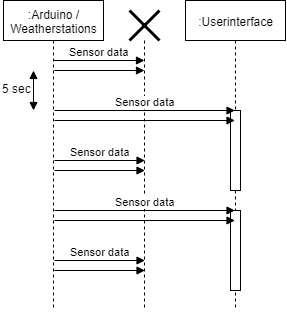
\includegraphics[width=0.4\textwidth, angle =0]{Struktureret_System_Udvikling/Workshop_2/Assets/Workshop2_SequenceDiagram.png}
    \caption{Interaction Sequence Diagram}
    \label{fig:my_label}
\end{figure}
\noindent
Vejrstationens opgave er, som vist ovenfor, at sende data hvert femte sekund, uden hensyntagen til nogen modtager. Modtageren "Userinterface" tager nemlig selv initiativ til, efter rådighed, at modtage og bearbejde den tilgængelige data.
Dette gør at data ikke bare er tilgængelig for den enkelte modtager men istedet for alle interesserede.
Til transformation af Data mellem Vejrstation og Userinterface, har gruppen valgt at opbygge følgende API:
\begin{figure}[H]
    \centering
    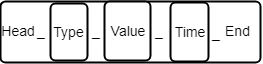
\includegraphics[width=0.3\textwidth, angle =0]{Struktureret_System_Udvikling/Workshop_2/Assets/Workshop2_DataStructure.png}
    \caption{Data Structure Blok}
    \label{fig:my_label}
\end{figure}
\noindent
Denne opbygger en struktur, der generelt kan indeholde alle typer af Vejrstationens sensor data, skelnet mellem ved datablokkens type blok.

% Hvordan kan man tilføre en ny sensor? Det kan man ved at lave en ny klasse som igen nedarver fra "Measurement_Module" med et nyt unikt type ID. Der udover skal PC siden også opdateres med hvordan denne nye type data skal fortolkes når den skal vises. Altså skal Display_Handleren også opdateres med håndteringen af den nye type data

\section{Modularitet}
Systemet er designet så yderligere sensorer kan integreres med mindst mulig ændring i koden. Hvis en ny sensor skulle integreres ville det være nødvendigt at oprette en ny klasse som nedarver fra \textit{Measurement\_Module}. Denne nye klasse vil så skulle læse data fra sensoren og sætte \textit{Type} variablen til et nyt unikt ID, eksempelvis 2, da 0 og 1 allerede er brugt. Den næste ændring vil være i \textit{Display\_Handler} klassen. Dette er nødvendigt for, at den kan display målingerne som værende fra denne nye sensor. Hvis ikke dette tilføjes, vil den blot modtage data med en ukendt \textit{Type}, vil den dermed ikke fungere.